\section{Calculating susceptibility}
    \label{Sec:Exp:Susceptibility}

Code to calculate the Lindhard susceptibility was written in MATLAB (Appendix \ref{Appendix:SusceptibilityCode} contains the full code) and early versions were tested with free electron cases in 2 and 3 dimensions with results shown in \fig\ref{Fig:Exp:FreeElectronSusceptibility}. This matches the expected free electron curves\footnote{See, for example, page 126 and Appendix F of reference\cite{Dressel2002}}. One caveat when dealing with the free electron case is that the energy dispersion is not periodic and as such needs to be truncated at some point in a spherically symmetric way. This truncation affects the final calculation but provided it occurs far enough from the Fermi surface then the difference is minimal. The results shown are for a calculated region that was a sphere of radius 1 with a Fermi surface radius of 0.3. Values for $\delta$(=1e-9) and $\omega$(=1e-9) are somewhat arbitrary given that the dispersion is simplified with $\hbar^2/2m = 1$ but are given here for posterity. 

\begin{figure}[htbp]
    \begin{center}
        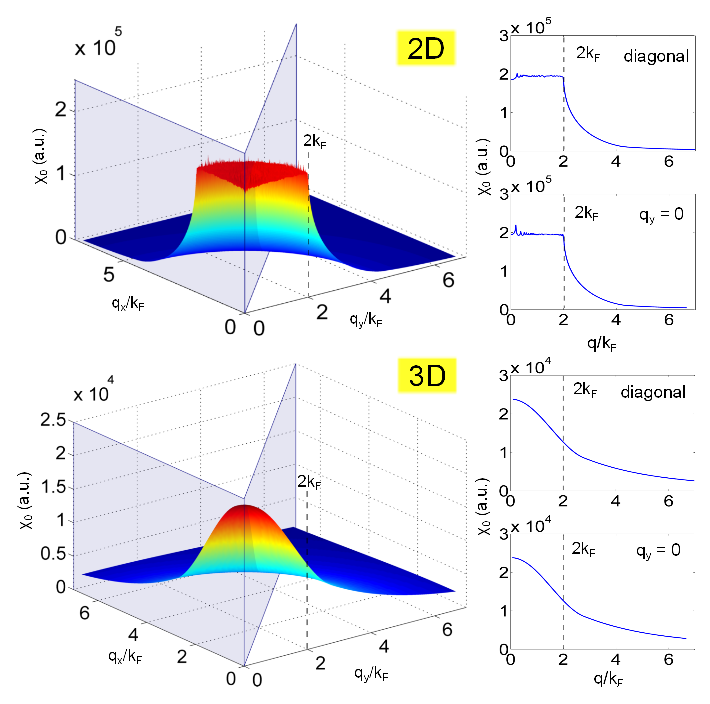
\includegraphics[scale=0.9]{Chapter-dHvABaFe2P2/Figures/AngleDepMeasurements/SusceptibilityFreeElectron/SusceptibilityFreeElectron}
        \caption{The real part of the Lindhard susceptibility calculations for a free electron model at $T=\unit[0]{K}$ using the MATLAB \code{calc_x0.m} code. Top panels are for the 2D case over a $500\times500$ point grid, the bottom panels are for the 3D case taken over a $100\times100\times100$ point grid. Panels to the right correspond to slices through the surface plots on the left. Calculations in the 3D case are at $q_z=0$.}
        \label{Fig:Exp:FreeElectronSusceptibility}
    \end{center}
\end{figure}


The code was adapted to accept pre-generated energy dispersions as calculated with the WIEN2k DFT software and post-processed with Ed's MATLAB code. In this case, the dispersion is periodic and energies at the scattering vector $q$ are obtained by simply `rolling' the 3D matrix of energy values. Testing on this adapted code was performed by re-creating WIEN2k calculations on LaFeAsO$_{0.1}$F$_{0.9}$ performed by Mazin et al.\cite{Mazin2008} and then comparing our own susceptibility calculations with those in the Mazin paper. A temperature smearing of \unit[1]{mRy} was quoted which was equated, using the Boltzman conversion, to a temperature of \unit[157.88]{K}. A similar amount of points ($55\times55\times26$) was also used. The result of the WIEN2k calculations are almost exactly equivelent as is evident in the comparisons of the spaghetti plots in top panels of \fig\ref{Fig:Exp:MazinX0Comparison}. The spacing of the points in the spaghetti plot is indicative of the courseness of the energy grid and by fitting a parabola energy dispersion (shown in orange) we can understand, approximately, the magnitudes of the effects of temperature ($T$), quasiparticle lifetime ($\delta$) and the frequency of the perturbing field ($\omega$) on the Lindhard susceptibilty, all of which will be discussed later. The lower panels of \fig\ref{Fig:Exp:MazinX0Comparison} show comparisons of $\Re\chi_0(q,\omega)$ and $\Im\chi_0(q,\omega)$ with the published results. For these calculations the values of $\delta=\textrm{1e-4}$ and $\omega=\textrm{1e-6}$ were determined to give the closest results from a series of trials\footnote{There is no indication in the paper as to the values of $\delta$ and $\omega$ used in their own calculations although we know that they are likely to be of the order of the temperature energy scale (\unit[1]{mRy}) or less.}. The comparison shows that some of the finer structure from the Mazin paper is missing from our own calculations, for example the depression in the real part at the $\Gamma$ point, however the overall shape is very similar.

\begin{figure}[htbp]
    \begin{center}
        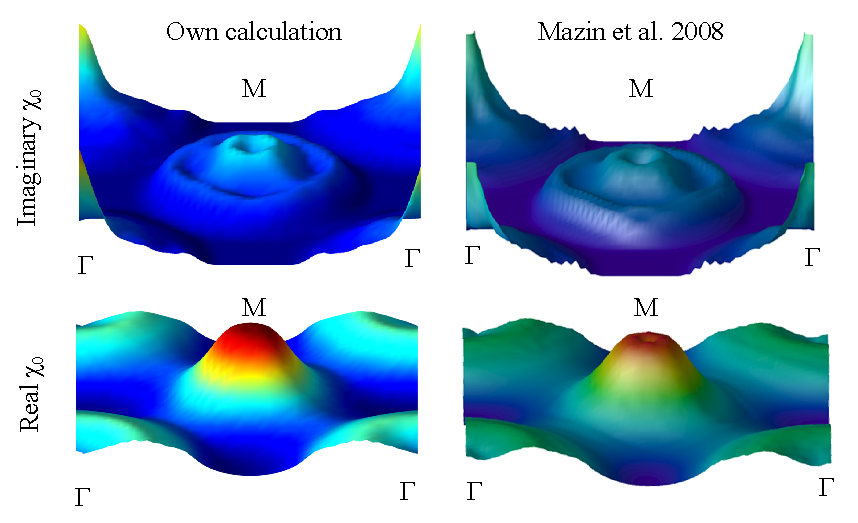
\includegraphics[scale=0.9]{Chapter-dHvABaFe2P2/Figures/AngleDepMeasurements/SusceptibilityMazinComparison/SusceptibilityMazinComparison}
        \caption{Right hand panels show the real and imaginary parts of Lindhard susceptibility calculations on LaFeAsO$_{0.1}$F$_{0.9}$ by Mazin et al. for $q_z=\pi/c$, right panels show the same calculation performed using our own MATLAB code.}
        \label{Fig:Exp:MazinX0Comparison}
    \end{center}
\end{figure}

Applying a temeprature smearing to the function is useful to gloss over the finite element size in the calculation which can cause significant spikes in the results. \Fig\ref{Fig:Exp:SusceptibilityTempSmearing} shows the smearing at particular temperatures. The choice of temperature depends on the granularity of your model as well as the expected fine detail of the results. For our calculations a temperature of \unit[158]{K} was used which corresponds to \unit[1]{mRy} which was the smearing used in a similar investigation into LaFeAsO using a comparable number of data points\cite{Mazin2008}.

\begin{figure}[htbp]
    \begin{center}
        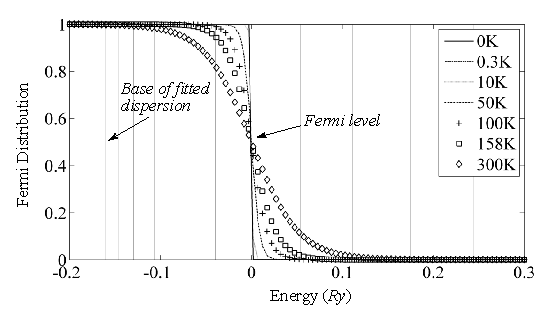
\includegraphics[scale=0.9]{Chapter-dHvABaFe2P2/Figures/AngleDepMeasurements/SusceptibilityTempSmearing/SusceptibilityTempSmearing}
        \caption{The Fermi distribution plotted at various temperatures using a contrived free electron distribution of energies scaled to the results of band 1 DFT calculations. An arbitrary Fermi energy of \unit[0.6]{Ry} is shown. The vertical lines shown the distribution of points in the model and are to illustrate the amount of smearing over points in the model that occur.}
        \label{Fig:Exp:SusceptibilityTempSmearing}
    \end{center}
\end{figure}

